%\chapter{Improving VoIP QoE in the Face of Large Decision Spaces}
\chapter{Tackling Large Decision Spaces}
\label{ch:via}


%\providecommand{\cmark}{\ding{51}}%
%\providecommand{\xmark}{\ding{55}}%

\providecommand{\ControlPlane}{{video optimization system}\xspace}
\providecommand{\mdn}{{MDN}\xspace}
\providecommand{\managed}{{managed overlay network}\xspace}
\providecommand{\Managed}{{Managed overlay network}\xspace}
\providecommand{\voip}{{audio conference application}\xspace}
\providecommand{\Voip}{{Audio conference application}\xspace}


%\providecommand{\skype}{{\sf\small Anon}\xspace}
\providecommand{\skype}{{Skype}\xspace}
\providecommand{\azure}{{ABC}\xspace}
\providecommand{\direct}{{default}\xspace}
\providecommand{\option}{{relaying option}\xspace}
\providecommand{\options}{{relaying options}\xspace}


The previous chapters have largely focused on addressing 
system and algorithmic challenges resulting from a complex relationship between 
session-level features and QoE.
In this chapter, we examine another
challenge caused by {\em large decision spaces}.
As we will see, this challenge is especially salient in Internet telephony.
%and solutions for applying \ddn paradigm
%In this chapter, we demonstrate the opportunities of \ddn paradigm in 
%another application--Internet telephony. 

In this chapter, to alleviate call quality problems shown in Section~\ref{sec:measurement:voip},
we present an architecture called \hybrid, which revisits the use of 
classical overlay techniques to relay calls with the emerging architecture of
managed overlay network. 
Trace-driven analysis shows that an oracle-based managed overlay can
{\em potentially} improve up to $53\%$ of calls whose quality 
is impacted by poor network performance. 
It is tempting to realize this potential improvement by using a \ddn-based
solution similar to Pytheas, but there is a unique practical challenge 
in the face of  a large number of relaying choices. 

To address the new challenge, we develop a practical relay selection system
that intelligently combines prediction-based filtering with an online 
exploration-exploitation strategy. 
The key insight is that the decision space
can be reduced by leveraging the persistent structures that 
for each pair of caller AS and callee AS, there is a small 
and stable subset of promising relays that contains the best one.
%We develop a practical relay selection approach that  
%intelligently combines prediction-based filtering with an online exploration-exploitation strategy. 
Trace-driven analysis and a small-scale deployment 
shows that \hybrid cuts the incidence of poor network 
conditions for calls by $45\%$ (and for some countries 
and ASes by over $80\%$) while staying within a budget
for relaying traffic through the managed network.


%In addition to demonstrating the opportunities of \ddn in improving
%VoIP QoE, we identify a unique challenge that Internet telephony has 
%more data sparsity due to a larger decision space. To address
%the new challenge, we present a novel system to reduce the 
%decision space by leveraging the persistent structures that there
%is 
%
%In Section~\ref{sec:measurement:voip}, we observe that
%call quality problems are quite pervasive. More importantly,
%these problems are significantly spread out geographically
%and over time, thereby making simple fixes targeted at specific
%``pockets'' of poor performance largely ineffective.
%
%To alleviate call quality problems, we present an architecture called \hybrid that  revisits the use of classical overlay techniques to relay calls. We argue that this approach is both timely and pragmatic given the emergence of private backbones in recent years to connect globally distributed datacenters, which can serve as a readily available infrastructure for a {\em managed} overlay network. Trace-driven analysis shows that an oracle-based overlay can {\em potentially} improve up to $53\%$ of calls whose quality is impacted by poor network performance. A key challenge is realizing these benefits in practice, in the face of significant spatial and temporal variability in performance and a large number of relaying choices. We develop a practical relay selection approach that  intelligently combines prediction-based filtering with an online exploration-exploitation strategy. Trace-driven analysis and a small-scale deployment shows that \hybrid cuts the incidence of poor network conditions for calls by $45\%$ (and for some countries and ASes by over $80\%$) while staying within a budget for relaying traffic through the managed network.


This chapter is organized as follows.
We begin by describing the architecture of relay selection in Internet telephony in Section~\ref{sec:via:arch}, and quantify the potential benefits of a managed overlay
network for improving audio call quality in Section~\ref{sec:via:potential}.
Then in Section~\ref{sec:via:design}, we then highlight the challenges in achieving these benefits and present 
a practical relay selection algorithm
that delivers close-to-optimal performance.
Section~\ref{sec:via:eval} uses simulation driven by real-traffic measurement and shows 
that VIA can significantly improve
Skype performance on network metrics.
Finally, we discuss related work in Section~\ref{sec:via:related}, and 
summarize the section in Section~\ref{sec:via:summary}.

\section{VIA Architecture}
\label{sec:via:arch}

\begin{figure}[t!]
\centering
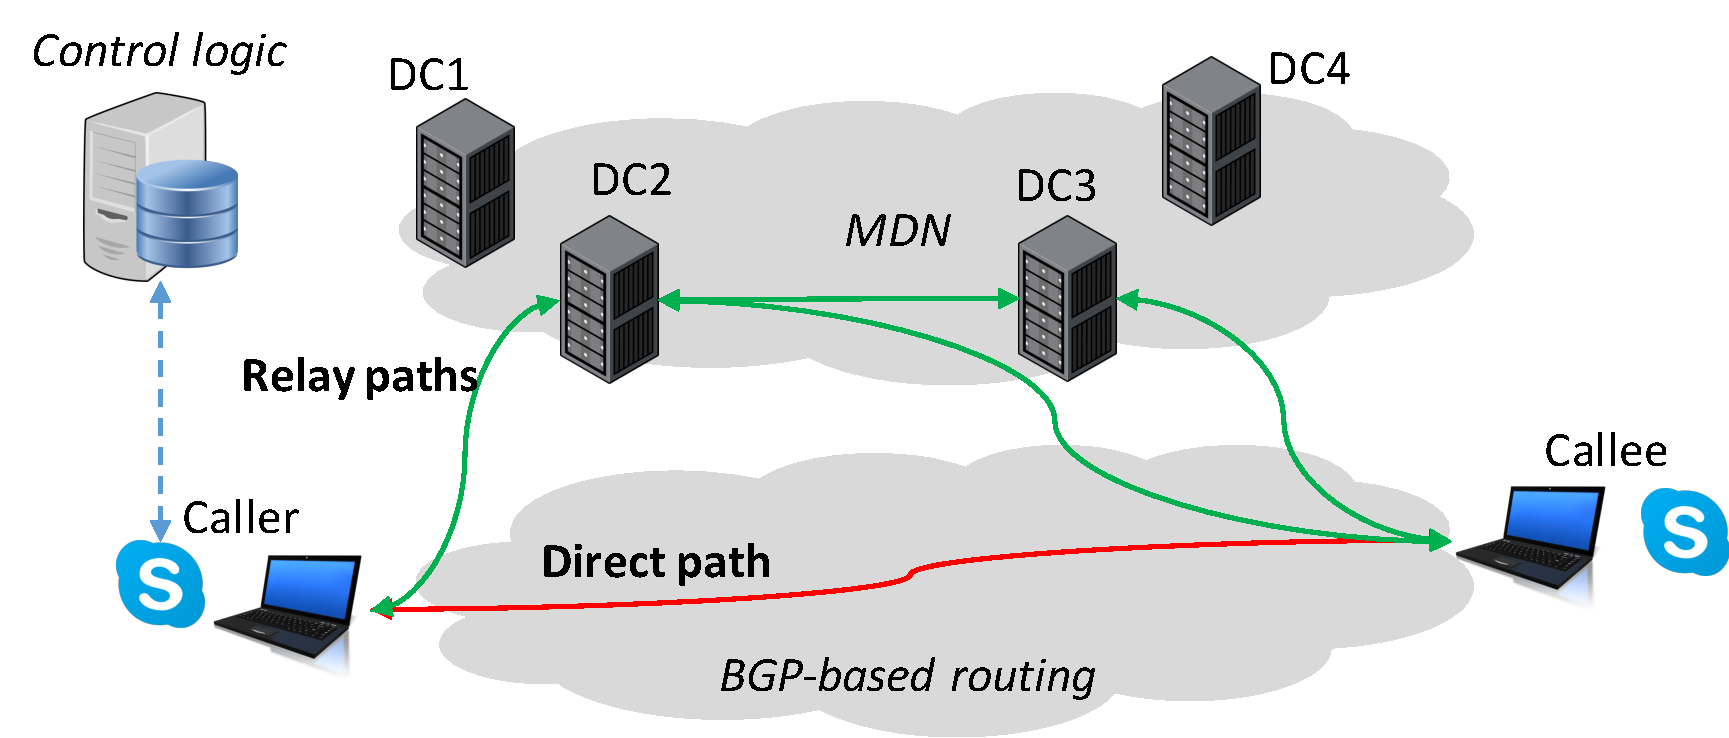
\includegraphics[width=0.7\textwidth]{figures/Via-MdnOverview.pdf}
\caption{\hybrid architecture with relay nodes at globally distributed data centers. A call can either take ``\direct path'' (red) or a ``relay path'' (green).}
%\ga{Callee to controller line.}
\label{fig:mdn-overview}
\end{figure}

Figure~\ref{fig:mdn-overview} presents the \hybrid architecture that consists of relay nodes placed at globally distributed datacenters, such as those run by Amazon, Google, and Microsoft. 
Indeed, {\hybrid}'s architecture bears similarities to those used by Google Hangouts and Skype~\cite{VideoTelephony-IMC12}, but with a key difference --- today, the relays are typically used to provide connectivity between any two clients, while \hybrid is engineered to {\em explicitly} optimize network performance and call quality.
%Indeed, this architecture bears similarities to that used by Google Hangouts and Skype~\cite{VideoTelephony-IMC12}, albeit primarily for connectivity (i.e., firewall and NAT traversal) rather than performance optimization (which is our focus here).

Each call can take either the ``{\em \direct} path'' (red arrow) or a ``{\em relayed} path'' (green arrows) that routes the traffic through one or more relay nodes in the DCs. Relayed paths could include a single relay to "{\em bounce} off" traffic or a pair of relays to enable traffic to "{\em transit} through" the private backbone of the managed overlay network. 


%%%%In our study, we use $74$ relay nodes, all located in a single AS\camera{ (so all inter-relay paths are across a private WAN)} and operated by \skype but spread across large datacenters and edge clusters in $30$ countries across $5$ continents. 
In our study, we use all the relay nodes operated by \skype. They are all located in a single AS (so all inter-relay paths are within a private WAN) but spread across many tens of datacenters and edge clusters worldwide. 
We assume the caller (or callee) can reach these relays %either through a shared anycast address, by letting the underlying network routing pick the "closest" relay, or 
by explicitly addressing the particular relay(s). %\camera{In this work, we assume the latter.} %\vnp{I'm confused by the previous sentence --- isn't Via all about explicitly selecting the relays?}
%In any case, since the relays are all in the same AS, the inter-domain path is determined by BGP. 
The network path between a relay and a client is determined by BGP. 
%While we could have considered approaches such as having a regionally-advertised IP block for each relay, to enable greater control over the {\em path} to each relay, we explicitly avoided these for ease of deployment.\vnp{The previous sentence can be deleted if we need to save space}

% Relaying audio calls through a \managed is feasible and is likely to provide better performance than BGP on international and interdomain calls, since large entities such as Amazon and Microsoft own geo-distributed DCs and edge clusters with high-quality backbone connectivity between them.

% The architecture in Figure~\ref{fig:mdn-overview} is generic and bear many similarities to the one that is being operated by Google Hangouts and Skype~\cite{imc-skype-study}. Based on data from \skype, we use $74$ relay nodes that are located across large datacenters and edge clusters, spread over \fillme countries. 

% Relayed calls typically traverse two relay nodes. The packets from the caller enter the \managed via a (nearby) {\em ingress} relay node, which in turn routes the packet via the private backbone to an egress relay that is close to the callee. Transparent to both the end-points, the call might internally traverse other relay nodes. Depending on the network characteristics, calls might also be {\em bounced off} just a single relay. The route between the end-points and the relays is either via anycast (wherein a common addressed is advertised from all the peering locations) or by explicitly picking from a set of regionally-advertised IP addresses, each corresponding to a specific relay. We explicitly avoided approaches that require control of the path to the relay for ease of deployability.

When establishing a call, after the caller signals its callee, both the caller and callee contact a {\em controller} (Figure~\ref{fig:mdn-overview}) to determine whether they should use the direct path or a relayed path, and, in case of the latter, which relay(s) they should use. The controller makes this decision based on the performance measurements from historical calls and policy constraints (such as those based on relay budget or current load), to be described in Section~\ref{sec:via:design}. To aid in this process, \skype clients periodically push the network metrics derived from their calls, to the controller. 
%As Section~\ref{sec:motivation} motivated, the controller dynamically updates its decisions using the latest measurements. 

The controller does not need to directly monitor the relay nodes because their performance (including degradation and failure) would be reflected in the end-to-end measurements made by clients who use the relays. %\footnote{In addition to the end-to-end measurements, we also rely on network performance measurements between the relay nodes, as explained in \Section~\ref{subsec:potential-overall}}.}
To avoid overloading the controller, each client could cache the relaying decisions and refresh periodically though we do not consider this here. (We 
 discuss implementation issues in Section~\ref{sec:via:discussion}). %in this paper.
%\ga{Cache results to avoid going to the controller?}
% , and returns as output the selection of relay or direct path for each call. 
%A naive control logic would be to have all calls relayed through the same relay nodes. However, since many BGP paths only have quality issues for a small fraction of time (see Figure~\ref{fig:temporal-structure}), it would be desirable to have a dynamic decision algorithm that select paths depending on when and between which nodes a call is being placed.


\section{Potential Relaying Improvement}
\label{sec:via:potential}

%Overlay routing is a well-studied topic, with over a decade of research and measurement studies~\cite{XXX}. While its benefits have been demonstrated in relatively small-scale and controlled settings (e.g., dozens of end nodes, which also doubled up as relays, typically located in university networks or research testbeds such as PlanetLab), we report results from the {\em first large-scale study of the potential benefits of overlay routing in a production setting the wild}, using the dataset of VoIP calls from a large production service, \skype.  
%We report results from the {\em first large-scale study of the potential benefits of relaying on Internet telephony}, using the dataset of VoIP calls from the \skype service.  


Next, we quantify the potential gains of \hybrid, using an ``oracle'' control logic, which enjoys the benefit of foresight. For each call between a source-destination pair, it has knowledge of the average performance of each {\em \option} on a given day. As shown in Figure~\ref{fig:mdn-overview}, a \option could be either the \direct (direct) path, a bouncing relay path, or a transit relay path.
For each source-destination pair, the oracle picks the \option that has the best average performance (i.e., lowest RTT, loss rate, or jitter) for this source-destination pair on this day--- either a relay path or the direct path.\footnote{Picking a day's granularity gives us sufficient samples for most of the \options. Nevertheless, for the small fraction of source-destination pairs for which we had sufficient samples {on a timescale of minutes}, we found that the oracle still had a significant benefit.} We also have information from \skype on the RTT, loss and jitter between their relay nodes, which we use in estimating the performance of a transit relay path. 

%noticed that the oracle's decisions were reasonable similar to its decisions using the average values over the day.% were reasonably similar. \vnp{vague!}} 
The oracle makes two simplifying assumptions: (1) there are no load restrictions on the relays or the network backbone, and (2) the performance measurements of each \option are indicative samples of its actual performance.
In Section~\ref{subsec:practical-budget}, we will relax the first assumption by introducing a budget constraint on the fraction of calls being relayed.
%the performance estimates of a call the oracle decides to relay is drawn from the distribution of call samples via the chosen relay. \vnp{I don't understand (2)}

\begin{figure}[t!]
\centering
%\hspace{-0.5cm}
\subfloat[\small{Performance distribution}]
{
        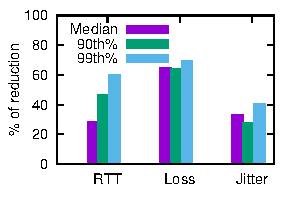
\includegraphics[width=0.45\textwidth]{figures/Via-Potential-Bar-Overall-MinChoices-5-Performance.pdf}
        \label{subfig:perf}
}
%\hspace{-0.5cm}
\subfloat[\small{Poor Network Rate}]
{
        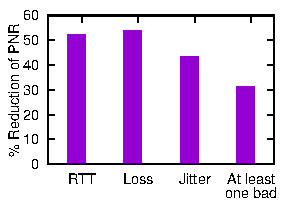
\includegraphics[width=0.45\textwidth]{figures/Via-Potential-Bar-Overall-MinChoices-5-PNR.pdf}
        \label{subfig:pnr}
}
%\hspace{-0.5cm}
%\hspace{-0.5cm}
%\subfigure[RTT]
%{
%        \includegraphics[width=0.24\textwidth]{new-figs/Potential-CDF-MinChoices-5-rRTT.pdf}
%        \label{subfig:}
%}\hspace{-0.5cm}
%\subfigure[Loss rate]
%{
%        \includegraphics[width=0.24\textwidth]{new-figs/Potential-CDF-MinChoices-5-rLOSS.pdf}
%        \label{subfig:}
%}\hspace{-0.5cm} \\
%\hspace{-0.5cm}
%\subfigure[Jitter]
%{
%        \includegraphics[width=0.24\textwidth]{new-figs/Potential-CDF-MinChoices-5-rJITTER.pdf}
%        \label{subfig:}
%}\hspace{-0.5cm}
%\subfigure[PNR]
%{
%        \includegraphics[width=0.24\textwidth]{new-figs/Potential-Bar-Overall-MinChoices-5.pdf}
%        \label{subfig:}
%}\hspace{-0.5cm}
\caption{Potential improvement of \hybrid.}
\label{fig:potential-percentile}
\end{figure}


%\begin{figure}[t!]
%\centering
%\includegraphics[width=0.4\textwidth]{new-figs/Improvement-Overall.pdf}
%\tightcaption{Improvement on mean, 90th, 99th percentiles and poor network rate (PNR) of RTT, loss and jitter. The relay path is selected for each AS pair to optimize individual metrics. 
%We also shows the fraction of reduction on fraction of calls with at least one metric being bad. }
%\label{fig:potential-percentile}
%\end{figure}

\mypara{Gains from oracle approach} Figure~\ref{fig:potential-percentile} shows the improvement (i.e., reduction) in the values of RTT, loss and jitter individually as well as the PNR (defined in Section~\ref{subsec:measurement:voip:method}). Specifically, if 
% the values in the dataset currently and after our decisions are
a statistic goes from  $b$ to $a$, we define the {{\em relative}} improvement as $100 \times (\frac{b-a}{b})$, which lies between $0$ and $100$. %\vnp{I presume Fig 9(a) shows the percentage reduction in the actual metrics, and Fig 9(b) the reduction in the PNR. If this is incorrect, the text here as also at the beginning of Sec 3 needs to be edited accordingly.}
%For each AS pair, we select the relay path to optimize individual metrics. The distribution of resulting performance is obtained by combining real performance measurements of the path picked for each AS pair and weighted by the population of each AS pair. 

The oracle can help reduce RTT, loss and jitter by $30\%$-$60\%$ at median (Figure~\ref{subfig:perf}). Reduction at the tail, which is of particular significance in interactive services,
% importance in production, 
is nearly  $40\%$-$65\%$ with the oracle's choice of relaying. All this translates to a healthy reduction in the PNR on each of RTT, loss, and jitter (Figure~\ref{subfig:pnr}, left three bars) of up to $53\%$. Source-destination pairs with fewer calls between them have a lower impact on the PNR and its improvement. 

We also analyze the reduction in PNR when the three metrics are considered {\em together}, i.e., improving from a situation where at least one of the metrics is poor to a situation where {\em none} of the three is poor (i.e., RTT $\leq 320$ms, loss $\leq 1.2\%$, {\em and} jitter $\leq 12$ms), while still optimizing for RTT, loss and jitter individually. %This helps us understand how correlated is the improvement in the three metrics. 
Even while optimizing for each of the three metrics, we can obtain a PNR for ``at least one bad'' metric; we conservatively pick the {\em worst} among the three for our analysis. Despite this strict stipulation, we can achieve reduction of over $30\%$ in PNR (Figure~\ref{subfig:pnr}, right-most bar).

\begin{figure}[t!]
\centering
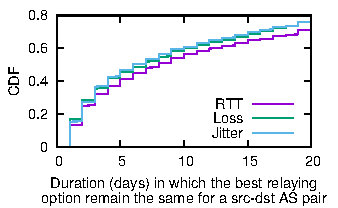
\includegraphics[width=0.5\textwidth]{figures/Via-Potential-PersistenceOfOracleDecision.pdf}
\caption{Distribution of how long the best \option (picked by oracle) lasts. The optimal \options for $30\%$ of AS pairs last for less than $2$ days.}
\label{fig:potential-persistence}
\end{figure}

\mypara{Need for dynamic relay selection} 
Whether the controller should select relay dynamically depends on how often the relaying decisions need to be updated. 
Figure~\ref{fig:potential-persistence} shows the distribution of the median duration during which the oracle picks the same \option for a source-destination AS pair.
%For each source-destination AS pair, persistence is defined by the median consecutive days during which oracle picks the same relay option. 
The optimal \option for $30\%$ of AS pairs lasts for less than $2$ days, and only $20\%$ of AS pairs have the same optimal relay option for more than $20$ days. 
This, together with the observation on the relatively low persistence of poor performance (Figure~\ref{fig:temporal-structure}), suggests that the relay selection should be done {\em dynamically}, rather than statically.



\section{VIA Relay Selection}
\label{sec:via:design}

Having shown that relaying through \hybrid could provide significant gains, 
we now devise a {\em practical} algorithm for relay selection. 
%In this section, we focus on the design of \hybrid's relay selection algorithm. 
 We begin by formulating the problem of relay selection. We describe 
 two classes of strawman approaches --- purely {\em predictive} and {\em exploration-based} ---
 and highlight limitations of both classes. We then present
 the core intuition behind our relay selection algorithm, called {\em prediction-guided exploration} and then describe 
 the solution. 

 
\subsection{Problem Formulation} 

Our goal  is to assign each call  to a particular \option as discussed in
Section~\ref{sec:via:arch}.  Recall that a \option can use the \direct
path, use a specific one-hop relay node (i.e., bouncing relaying), or use a specific pair of 
relay nodes (i.e., transit relaying).  Let  $\CallSet$ denote the set of calls we want to 
optimize and  let $\RelaySet$ denote the set of available \options. 
 We use $\Call \in \CallSet$ and   $\Relay \in
\RelaySet$ to denote a specific call and \option, respectively.
 Let $\QualityFunc(\Call, \Relay)$ denote the expected  
 {value of a network metric for} $\Call$  when using $\Relay$ {(a smaller value is better)}.
We assume that the relaying decisions for calls are independent; i.e., the performance of a call is not impacted by the relaying decisions made for other calls.

%We assume that the \hybrid framework has as input a a set of observed call records with
%measured performance metrics, $\HistoryCallSet$. Given $\HistoryCallSet$, 

The
goal of \hybrid is to  {\em assign} optimal \options
 for each $\Call \in \CallSet$. Let $\Assign:\CallSet \rightarrow \RelaySet$ denote 
 the assignment function output by some algorithm and 
 let $\Assign(\Call)$ be the \option assigned for call $\Call\in\CallSet$.
 Formally, our objective is to find  the optimal 
 assignment
 
\begin{displaymath}\arg\min_{\Assign \in \RelaySet^\CallSet}  \sum_{\Call\in\CallSet}\QualityFunc(\Call, \Assign(\Call))
\end{displaymath}

\noindent This is a minimization problem because a lower value is better for each of our network quality metrics $\QualityFunc$.

\subsection{Strawman Approaches}
\label{subsec:strawmen}

We can consider two classes of approaches for the optimal assignment of \options to calls:

\begin{enumerate}
%\vspace{-.05in}
\item  {\em Exploration-based:} One approach is to set aside a fraction of the 
 calls for measurement-based exploration of the performance of each possible relaying option for every source-destination pair.  
 For instance, for every AS-pair and every possible % one-hop/two-hop relaying, 
\option $\Relay$,
 we will explicitly use some of the calls to explore the option and measure the performance, 
  $\QualityFunc(\Call, \Relay)$.
  
%\vspace{-.05in}
\item  {\em Prediction-based:} An alternative to the exploration-based approach
 is to use the recent history  of observed call performance. Suppose, \hybrid has available as
 input  call records with measured performance $\HistoryCallSet$. Then, we can use
 suitable prediction algorithms  to 
 predict the performance $\QualityFunc(\Call, \Relay)$ for every combination, and select the option that has the best predicted performance.

\end{enumerate} 

Unfortunately, we observe in practice that both classes of approaches individually  have
very poor accuracy in predicting $\QualityFunc(\Call,
\Relay)$. This  ultimately results in a poor assignment strategy and poor call
quality.  There are two key reasons. 

First, there is  a fundamental problem because of {\em skew in data
density.} Specifically, there is a substantial difference in the number of
call samples available across different source-destination pairs, both for the
direct path and for the various relayed paths.  This variability arises because
of the large space of choices: $N$ end-points and $M$ relay strategies lead
to $O(N^2M)$ choices.  Furthermore, certain end-points make/receive
fewer calls, yielding fewer samples. Second, there is {\em inherent variability} in the observed performance.
Consequently, to estimate  $\QualityFunc(\Call, \Relay)$, we need  a
significant number of samples before the empirically observed values can
converge to the true values. 

The skew and the variability make prediction inaccurate and exploration ineffective and/or expensive (in terms of the effort to be expended).

%\sout{Note that these challenges have implications for both classes of approaches.  With 
% the prediction based approaches, skew implies that there will be some 
% coverage ``holes'' in the prediction-based approaches while the exploration-based 
% approaches may not have sufficient calls to explore all relay choices. \ga{Unclear.}
% Similarly, the noise induced by variability means that the prediction-based approaches
% can easily miss the optimal relaying strategy and the exploration-based approaches
% will need a substantial measurement budget to converge.} 


\begin{figure}[t!]
\centering
%\includegraphics[width=0.4\textwidth]{ppt-figs/Overview.png}
%\includegraphics[width=0.5\textwidth]{ppt-figs/Overview-new.pdf}
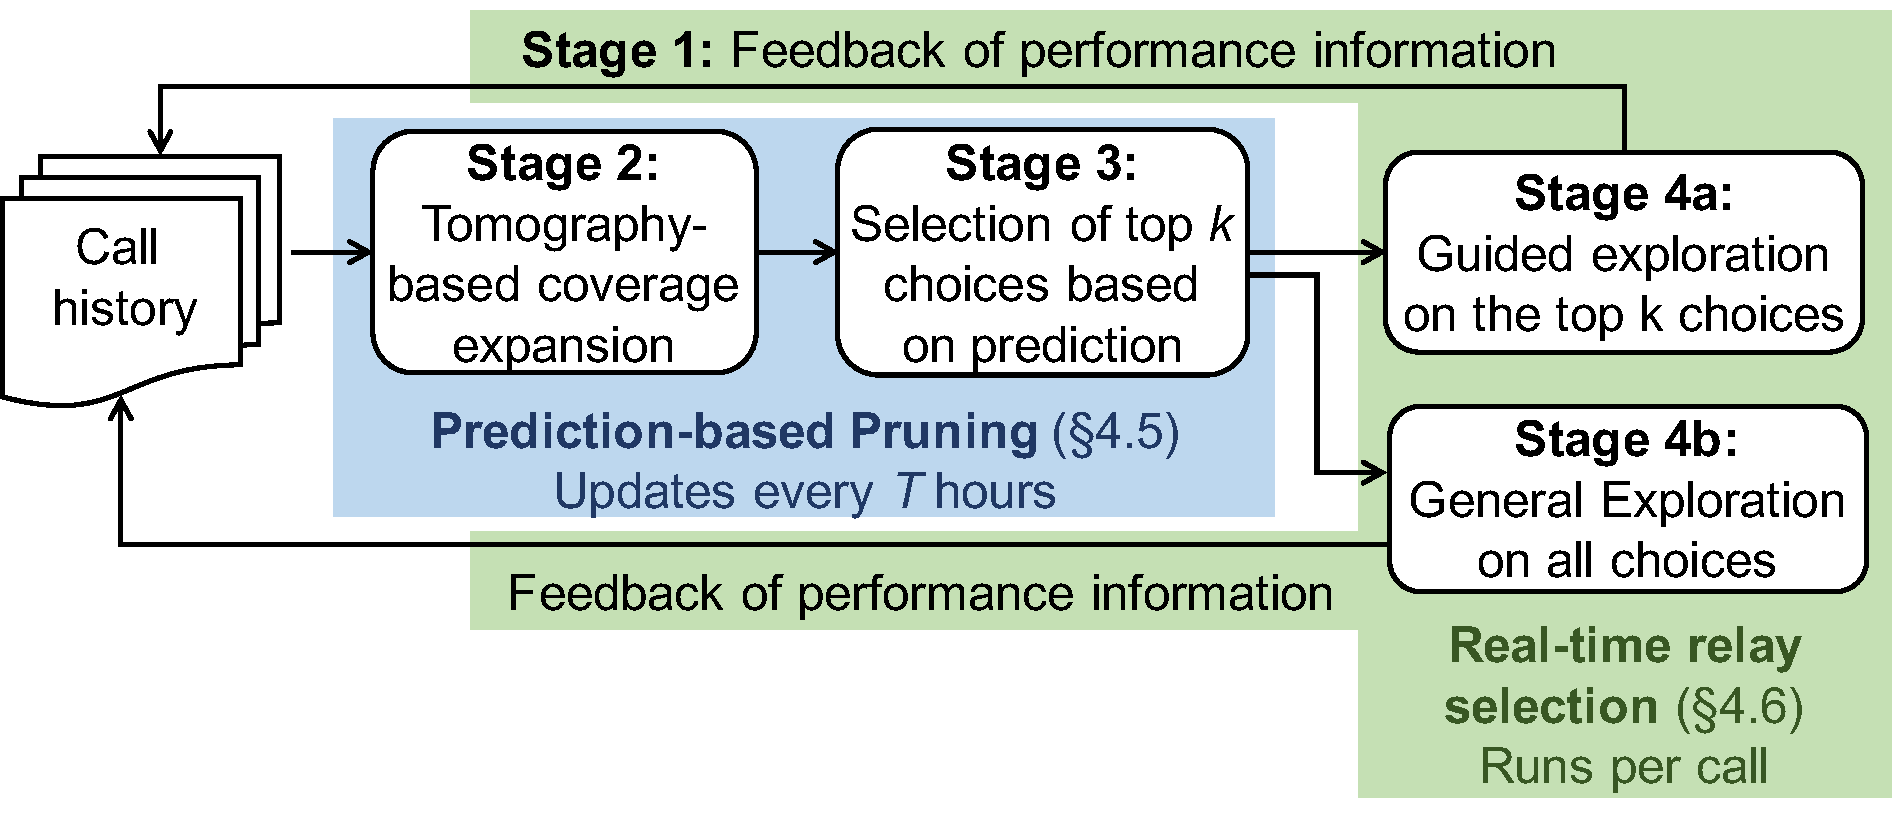
\includegraphics[width=0.5\textwidth]{figures/Via-Overview-new-ethan.pdf}
%\vspace{-0.5cm}
\caption{Overview of \hybrid relay selection based on prediction-guided exploration.}
\label{fig:intuition}
\end{figure}

%\subsection{Intuition behind our approach}
\subsection{Overview of \hybrid}
\label{subsec:Via-approach}

The key intuition behind our solution is the empirical observation that even though a prediction-based approach 
may not predict the optimal choice, the optimal is likely in the top few of its predictions. In other words, if we look at the top-$k$ choices 
(those who have the best predicted performances), the optimal choice will likely be a member of that set.%, even though it is a small subset of all possible \options $\RelaySet$. 
%may miss finding the true  optimal choice
%$\Relay^* = \arg\min_{\Relay \in RelaySet} \QualityFunc(\Call, \Relay)$, its
%prediction for that optimal choice 
%$\mathit{Prediction}(\QualityFunc(\Call, \Relay^*))$ is not too far away
%from the actual optimal value. A  natural corollary of  this observation is
%that if we look at a small number ($\leq 3$)   of top-k choices suggested by
%the prediction approach, then with high probability the true optimal strategy will be a member of
%that set; i.e., $\Relay^* \in \mathit{TopKPredictions}(\Call,k), k \leq 3$. 


We can exploit this observation to {\em prune} the search space for our
exploration  step. That is, the exploration approach does not need to blindly
explore the set   $\RelaySet$ of all possible strategies, but instead can focus
on a much smaller set of top-$k$ predictions.  We refer to this as a {\em
prediction-guided exploration}  approach.  
The top-$k$ pruning is not to be confused with a similar machine learning problem which seeks to find $k$ best options (e.g.,~\cite{cao2015top}). In contrast, we care more about the best \option {} -- our top-$k$ candidates may have bad options, but the best \option is very likely to be among them, and can be found by exploration techniques.

% Next, we describe the detailed design of the \hybrid approach
% for selecting the optimal relaying strategy. Algorithm~\ref{alg:hybrid} shows the psuedocode of \hybrid.


%\subsection{Overview of the \hybrid relay selection}
%\label{subsec:Via-approach}

Figure~\ref{fig:intuition} depicts the main stages in \hybrid, and Algorithm~\ref{alg:hybrid} shows the pseudocode. In a nutshell, the logical stages are: 
\begin{enumerate}
\item gathering performance information from call history, %\vspace{-.05in}
\item using network tomography to expand the coverage of the information from call history, %\vspace{-.05in}
\item using the (expanded) history information to predict performance and prune all but the most promising top-$k$ \options, and %\vspace{-.05in}
\item perform exploration-exploitation on the top-$k$ \options as well as all \options using multi-armed bandit (MAB) techniques.
\end{enumerate}

Finally, the observed performance of each call will be stored in call history, i.e., fed back to stage $1$.
Stages $2$ and $3$ (shown in light blue) %\vnp{the camera-ready paper will be in b\&w,so better to use a different method of highlighting} 
are performed at a periodicity of $T$ hours (by default $24$ hours), i.e., the pruned list of candidate \options are refreshed every $T$ hours.  Stages $1$ and $4$ (shown in light green) are performed on a per-call basis.
We discuss these stages in the sub-sections that follow.

\SetAlgoNoLine
\begin{algorithm}[t!]
\begin{small}
\nonl\hrulefill

\KwIn{Set of calls $\CallSet$ to be assigned to \options $\RelaySet$, and set of historical calls $\HistoryCallSet$}
\KwOut{A relay assignment, $\Assign$, where each call $\Call\in\CallSet$ is assigned a relay option $\Assign(\Call)\in\RelaySet$}

\nonl\hrulefill

%\red{Apply tomography to expand coverage of $\HistoryCallSet$}
\tcc{\scriptsize Stage 2: Tomography-based performance predictor trained from \HistoryCallSet}
$\Predictor\leftarrow \BuildPredictor(\HistoryCallSet)$

\tcc{\scriptsize Stage 3: Pick Top-$k$ candidates based on history-based prediction.}

$\Assign\leftarrow\emptyset$ 

\For{$(\Src,\Dst)$}{

	TopK$\leftarrow \GetTopK(\Src,\Dst,\RelaySet,\Predictor)$ 

	\tcc{\scriptsize See Algorithm~\ref{alg:pruning}}

	\For{$\Call\in\CallSet$}{

		\If{$RandomFloat(0,1) < \epsilon$}{
			\tcc{\scriptsize Stage 4a: Explore the Top-$k$ candidates}
			$\Relay\leftarrow\Explore(\Call,\Src,\Dst,\text{TopK},\Assign,\Predictor)$ 
		}\Else{
			\tcc{\scriptsize Stage 4b: Randomly explore all \options}
			$\Assign(\Call)\leftarrow Random(\RelaySet)$ 			
		}
		$\Assign(\Call)\leftarrow\Relay$ 
	}
}
\Return{\Assign} 

\nonl\hrulefill
\vspace{.1in}
\end{small}
\caption{\bf Relay selection algorithm of \hybrid}
\label{alg:hybrid}
\end{algorithm}


\subsection{Prediction-Based Pruning}
\label{subsec:practical-prediction}



% prediction, coverage vs. accuracy tradeoff
%The first step in \hybrid is to predict
Using call history data, \hybrid proceeds to predict, with confidence intervals, the performance between a source-destination pair over each \option:  direct paths, and each transit and  bouncing relay. %\vnp{"one-hop" and "two-hop" would be confusing, since it is actually 2 hops and 3 hops in the bouncing and transit cases, respectively} 

%\red{\noindent{\bf Expanding Coverage using Tomography:}
\mypara{Expanding coverage by network tomography}
Call history tells us the performance of paths that were actually used. 
As there is skew in call distribution, there might be ``holes'', i.e., no call history for the network path between a source-destination pair through a specific \option. 
Can we learn about the performance of these network paths? 
%Can we learn about the performance of network paths that are {\em not} contained in the history, e.g., one containing a relay not used before by a caller-callee pair? 

\begin{figure}[t!]
\centering
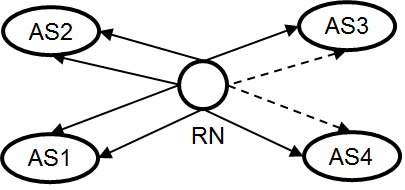
\includegraphics[width=0.4\textwidth]{figures/Via-Tomography.png}
\caption{Path stitching in \hybrid to estimate performance through relay RN. Solid lines represent historical call samples that we use to predict performance between AS$3$ and AS$4$ (dotted line). RTT$_{\text{AS3}\leftrightarrow\text{AS4}}$ $=$ RTT$_{\text{AS1}\leftrightarrow\text{AS4}}$ $+$ RTT$_{\text{AS2}\leftrightarrow\text{AS3}}$ $-$ RTT$_{\text{AS1}\leftrightarrow\text{AS2}}$.}
\label{fig:tomography}
\end{figure}

If we knew the performance of the individual network segments (e.g., client to relay) that comprise an end-to-end path, we could compose these to estimate the performance of the path. In principle, measurements of the individual network segments could be made by the relays themselves. However, the relays in \skype were only designed to forward traffic and we were not in a position to add new functionality to these relay nodes (and potentially impose additional overheads). 
%Nevertheless, how to leverage direct measurements between clients and relays, when they are available, is an area for future exploration.
%The situation is not unlike that in ISP networks where direct measurement of network links, while easy in principle, is challenging in practice, leading to indirect approaches for estimating such metrics as the link performance and the traffic matrix~\cite{tomo-gravity}.

 
Network tomography provides an alternative. By combining end-to-end measurements across several, partially-overlapping paths, network tomography can help estimate the performance of each network segment. Then, by stitching together the estimates for the individual segments, we can estimate the performance of a path not seen before.

Figure~\ref{fig:tomography} shows a simple example of how network tomography expands coverage. We use linear tomography, and apply it to individual 
%\cameraremove{which can be applied to }metrics that compose linearly (e.g., RTT) or can be linearized (e.g., jitter and packet loss rate, under the assumption of independence across network segments~\cite{Tomography-StatSci04}). 
%\camera{\footnote{While we make the assumption that the routing paths and performance metrics are symmetric on two directions this is fine because communication between the relays and clients are two-way and we only want the round-trip performance, not one-way performance.}}

%We model \BuildPredictor as a network tomography problem. 
Given a relay path that uses \option $\Relay$ and between source AS $\Src$ and destination AS $\Dst$, our tomography algorithm models it as a path consisting of two segments: a segment between $\Src$ and $\Relay$ and a segment between $\Dst$ and $\Relay$. 
Modeling network end-points on AS level is a pragmatic trade-off: it gives us sufficient data on many source-destination pairs, and still produce significant improvement (see Section~\ref{subsec:eval-parameter} for comparison between different granularities).
The prediction algorithm can work at a finer granularity (e.g., $/24$ IP prefix) when more data are available.



The $\Predictor$ module (Algorithm~\ref{alg:hybrid}, line $2$) predicts for a source-destination pair ($\Src$ and $\Dst$) both the mean performance $\Predictor_{mean}(\Src,\Dst,\Relay)$ for a specific \option $\Relay$, and its standard error of mean (SEM) $\Predictor_{sem}(\Src,\Dst,\Relay)$. %~\footnote{The standard error of mean is the standard deviation of a sample mean's estimate of the population mean. It tends to zero as the number of samples grows.}
Based on these, $\Predictor$ estimates both the lower and higher $95\%$ confidence bounds: $\Predictor_{lower}(\Src,\Dst,\Relay)=\Predictor_{mean}(\Src,\Dst,\Relay)-1.96\Predictor_{sem}(\Src,\Dst,\Relay)$ and $\Predictor_{upper}(\Src,\Dst,\Relay)=\Predictor_{mean}(\Src,\Dst,\Relay)+1.96\Predictor_{sem}(\Src,\Dst,\Relay)$.

%\commentout{
%\myparatight{Granularity:}
%Accordingly, we model {\sf\small BuildPredictor} as a network tomography problem. \red{A question, however, is at what granularity we should model the network.}
%%that takes the following inputs: performance measurements from the different end-hosts and network topology connecting the end-hosts (as obtained from, for example, traceroute measurements). The output of the tomography are performance values for each of the individual links in the network. With sufficient data, these individual link values can be, in principle, stitched together to obtain the expected performance between any given source-destination pair. \ga{Do we need more details?} 
%The finer the granularity, % of each of these components, 
%the lower the modeling error (since the underlying network would be modeled more faithfully) but the worse the statistical error and the poorer the coverage (since less data would be available). Here are a couple of examples of this trade-off:
%
%%\sout{the more the accuracy of the prediction. But it also comes the cost of fewer samples and hence lower coverage.} 
%
%
%\begin{enumerate}
%
%% spatial non-uniformity, topological options
%\item Network end-points and intermediate hops can be modeled at various granularities, such as fine-grained address blocks (e.g., /24 subnets) or a coarser AS level. At coarser granularities, there is an advantage of aggregation which results in many more call samples traversing each of the nodes and connected links. While this facilitates a statistically superior data-driven approach, it also introduces modeling errors, since an entire AS might be too large and heterogeneous to be modeled as a single node.\ga{Add illustrative figure.}
%
%\item The network topology connecting the end-points can either be coarse-grained like a star (where all end-points connect to a common hub) or a full-mesh (where the various pairs of end-points are connected directly to each other), or could include finer levels of detail such as % that consider all 
%the intermediate hops from the traceroute measurements. Again, the finer the granularity of the network topology, the greater its fidelity but less the data we get for each of the links, thereby affecting statistical confidence. %\vnp{Full-mesh presents a bit of a dilemma --- it has more links than traceroute but I would argue that it is neither more fine-grained or more faithful than traceroute. Hence the bit I have struck out.}
%
%\end{enumerate}
%
%% data-driven approach - combination
%We adopt a pure data-driven approach, wherein for each source-destination pair, we maintain the best combination of network topology and granularity that yields the most accurate prediction for each network metric. This combination is periodically updated as more performance samples (i.e., ground truth data points) are obtained from new calls. Our approach is scalable as each of these combinations can be computed independently, in parallel. 
%
%Such an adaptive data-driven approach deals better with the peculiarities of data collected in the wild (e.g., the availability of plentiful data for certain paths and little for others) than a one-size-fits-all approach. It beats the individual approaches (e.g., using only the traceroute topology) in its prediction accuracy handily.  %including doing only network tomography on traceroute topology. 
%Also, as our results presented in \fillme show, the various combinations of granularity and topology get widely exercised, justifying the data-driven approach.
%
%}

\mypara{Pruning to get top-$k$ choices} Pruning does not necessarily narrow down to the single best \option. However, we see that the best \option is often among the top-$k$ % of the
predicted options for a small value of $k$. For instance, the probability of the option with the minimum RTT being included even in top three or four ($k=3$ or $4$) is $60\%-80\%$ as against just $29\%$ if we were to pick only the option with the predicted minimal RTT ($k=1$). Therefore, we adopt the approach of using our predictor to pick the top-$k$ \options and use that for {\em guided exploration}.


%\begin{figure}[t!]
%\centering
%\includegraphics[width=0.4\textwidth]{ppt-figs/best-in-topk.pdf}
%\vspace{-0.3cm}
%\tightcaption{\camera{Probablity of best \option in the best $k$ \options chosen by prediction.}}
%\label{fig:top-k}
%\end{figure}

Instead of using a fixed value of $k$, \hybrid \ {\em dynamically decides} $k$ based on the lower and higher confidence bounds
%\cameraremove{the mean ($\mu_\Relay$) and standard error of mean ($\text{SEM}_\Relay$)} 
for each relay $\Relay$ on the particular source-destination pair $\Src$ and $\Dst$. Algorithm~\ref{alg:pruning} shows the pseudocode.
Specifically, we define top-$k$ to be the minimal set of \options such that the lower $95\%$ confidence bound ($\Predictor_{lower}(\Src,\Dst,\Relay)$) of any relay option not in the top-$k$ is higher than the upper $95\%$ confidence bound ($\Predictor_{upper}(\Src,\Dst,\Relay)$) of any relay option in the top-$k$. (Recall that the lower the value of a network metric, the better it is.) In other words, we are very sure that any relay option that is not included in the top-$k$ is worse than any that is. For instance, the probability of the option with minimal RTT being included in such top-$k$ is over $90\%$.


\SetAlgoNoLine
\begin{algorithm}[t!]
\begin{small}

\nonl\hrulefill

\KwIn{Source AS $\Src$, destination AS $\Dst$, \options $\RelaySet$, and predictor $\Predictor$ (from Algorithm~\ref{alg:hybrid})}
\KwOut{Top $k$ \options TopK for ($\Src$, $\Dst$) calls}

\nonl\hrulefill

\Fn{$\GetTopK(\Src,\Dst,\RelaySet,\Predictor)$}{
\tcc{\scriptsize Initializing variables}
TopK$\leftarrow\emptyset$; $\text{Remained}\leftarrow\RelaySet$; $h\leftarrow\infty$

\While{\textrm{true}}{
	$\Relay\leftarrow\argmin_{\Relay\in \text{Remained}}\Predictor_{\text{upper}}(\Src,\Dst,\Relay)$ 
	
	\If{$\Predictor_{\text{\text{lower}}}(\Src,\Dst,\Relay)>h$}{\textrm{\bf break} }
	\Else{
		$h\leftarrow\Predictor_{\text{high}}(\Src,\Dst,\Relay)$  
		$\text{Remained}\leftarrow \text{Remained}\setminus\{\Relay\}$ 
		$\text{TopK}\leftarrow \text{TopK}\cup\{\Relay\}$ 
	}
}
\KwRet{} TopK
}

\nonl\hrulefill

%\vspace{.1in}
\end{small}
 \caption{\bf Predicting the top-$k$ choices.}
\label{alg:pruning}
\end{algorithm}


\subsection{Exploration-Exploitation Step}
\label{subsec:practical-relaying}

Exploring the top-$k$ choices for each source-destination pair (\Explore of line $10$ in Algorithm~\ref{alg:hybrid}) can be formulated as an 
 instance of the classic multi-armed bandit problem, where each of the relaying options is an {``arm" of the bandit} and the network performance obtained is the ``reward''. While bandit selection is a much studied problem, doing so under high-variance and dynamically changing performance distributions (i.e., rewards) of the bandits, % high variance in their performance, 
and also limited budget for each bandit, requires interesting adaptations, as outlined below. 

Relay options selected by the basic {\em exploration-exploitation} process assigns a fraction of calls  to explore different relay options ($\epsilon$-greedy) and the rest to exploit the best decision.\footnote{Exploration-exploitation could also be invoked on per-packet basis within the call. However, this would require packet-level control, which is out of the scope of this paper.}
%Thus, the key of exploratory appraoch is to strike a balance between amount of calls used for exploration (i.e., reliably estimating performance of different paths) and exploitation (i.e., optimizing performance by using the best choice). 
As briefly mentioned earlier, standard exploratory approaches  are slow to converge (Section~\ref{subsec:strawmen}) and often fail to select the best decision (Section~\ref{subsec:design}). This is because exploring in presence of high variability requires a lot of samples, which is infeasible due to data sparseness and skew. %As Figure~\ref{fig:intuition} illustrates, without enough samples, basic exploratory selection suffers from non-convergence problem and has suboptimal performance.

Algorithm~\ref{alg:explore} shows the pseudocode of our approach.
 Here, we choose  the UCB1 algorithm~\cite{ucb1} as our 
 basic starting point. UCB1 is well-suited for our purpose because  
%\vnp{It seems to be from the following 2002 paper --- http://homes.di.unimi.it/~cesabian/Pubblicazioni/ml-02.pdf} 
 it does not require explicitly specifying the fraction of samples for exploration. Instead, it transparently combines both exploration as well as its exploitation decisions. % and works well for dynamic distributions. \vnp{This point about UCB1 working for "dynamic distributions" seems to contradict the "static" assumption noted below. I think we should delete the "dynamic distributions" bit.} 
 We make two modifications to the basic algorithm
 in order to make it work well in our context.


\SetAlgoNoLine
\begin{algorithm}[t!]
\begin{small}

\nonl\hrulefill

\KwIn{Call $\Call$, source AS $\Src$, destination AS $\Dst$, top $k$ \options TopK, relay assignment $\Assign$, predictor $\Predictor$}
\KwOut{Relay selection of $\Call$}

\nonl\hrulefill

\Fn{$\Explore(\Call,\Src,\Dst,TopK,\Assign,\Predictor)$}{
\tcc{\scriptsize Initializing variables}
$\text{ucb}_\text{min}\leftarrow \infty$; $\Relay_{\text{top}}\leftarrow\textrm{null}$ 

\tcc{\scriptsize To avoid outliers, we do not use maximum performance as normalizer $w$.}

$w\leftarrow\frac{1}{|\text{TopK}|}\sum_{\Relay\in \text{TopK}}(\Predictor_{\text{upper}}(\Src,\Dst,\Relay))$ 

\tcc{\scriptsize Following is the standard UCB1, except for the normalization scheme.}

$T\leftarrow|\Assign|+1$ 

\For{$\Relay\in \text{TopK}$}{
	$\CallSet_{\Relay}\leftarrow\{\Call' | \Assign(\Call')=\Relay\}$ 

	\tcc{\scriptsize$\QualityFunc$ is the quality function.}

	$\text{ucb}\leftarrow\frac{1}{w|\CallSet_{\Relay}|}\sum_{\Call'\in \CallSet_{\Relay}}\QualityFunc(\Call',\Relay)-\sqrt{\frac{0.1\log T}{|\CallSet_{\Relay}|}}$  

	\If{$\text{ucb}<\text{ucb}_\text{min}$}{
		$\Relay_{\text{top}}\leftarrow\Relay$

		$\text{ucb}_\text{min}\leftarrow \text{ucb}$ 
	}
}
%$\Assign(\Call)\leftarrow\Relay_{top}$ 
\KwRet{$\Relay_{top}$}
}

\nonl\hrulefill

%\vspace{.1in}
\end{small}
\caption{\bf Exploring the top-$k$ candidates in real time using modified UCB1.}
\label{alg:explore}
\end{algorithm}



\begin{enumerate}
%\vspace{-.05in}
\item UCB1 normalizes rewards (i.e., performance) from each bandit (i.e., relay option) to be between 0 and 1. In our situation, however, normalizing based on the full range of values of each performance metric is problematic due to 
	% to cope with 
the large variance in distribution % performance measurements 
(e.g., unusually large RTT). Normalizing all values based on such a wide range leads to poor decisions because the difference between values in the common case become hard to discern. Instead, we normalize the rewards by dividing them by the average of upper $95\%$ confidence bounds ($\Predictor_{upper}(\Src,\Dst,\Relay)$) of the top-$k$ candidates.%\vnp{Why average and not max?}

%\vspace{-.05in}
\item The top-k pruning in Section~\ref{subsec:practical-prediction} is a function of only the samples explored. Therefore, to avoid being blindsided by dynamically changing performance distributions, \hybrid also sets aside $\epsilon$ fraction of calls to random relays (outside of the top-$k$) for {\em general} exploration. This step is not required in traditional exploration-exploitation techniques as they assume the reward (performance) distribution of each bandit (relay option) is static, which may not hold % is not necessarily true 
in our context.
\end{enumerate}


\subsection{Budgeted Relaying}
\label{subsec:practical-budget}

%Having budget constraints means it does not suffice to identify only the optimal choice for a source-destination pair. We \red{may have} to assign calls to multiple relayed (or the direct) paths in order to meet the budget.
We extend {\hybrid}'s relaying decision to consider budget constraints: so the fraction of calls being relayed must be less than a certain limit, $\Budget$ (e.g., $30\%$). While such an overall budget on relayed calls is simple, in general it may also be of interest to consider other budget models, such as per-relay limits or bandwidth cap on call-related traffic. 
%According to the conversation with the production team of the large \voip provider, such budget constraint is realistic since \fillme. \vnp{Not sure we can provide hard justification, since the per-relay budget probably matters. Best to remove this last sentence, and replace it with something like "While here we only consider a limit on the aggregate fraction of relayed calls, in general it may also be of interest to consider per-relay limits.}

\hybrid utilizes the budget using a simple extension to the heuristic in Section~\ref{subsec:practical-relaying}. It decides to relay a call only if the benefit of relaying is {\em sufficiently} high. 
If the {overall} budget for relaying calls is $\Budget$ {percent}, a call should be relayed only if the benefit of relaying it is within the top $\Budget$ percentile of calls. 
\hybrid uses historical call information (of relaying benefits) to keep track of the percentiles. It decides to relay a call only if the expected benefit is above the $\Budget^\text{th}$ percentile benefit.
%Though the original \hybrid will relay a call as long as there is benefit, it can be easily modified to realize the above insight (shown in Algorithm~\ref{alg:budget}). \vnp{State in a sentence or two what the modication is.}






\section{Evaluation}
\label{sec:via:eval}

In this section, we show that \hybrid can significantly improve performance on network metrics.
Specifically, we show that:
\begin{packeditemize}
\item \hybrid achieves substantial improvement on all network metrics --- $20\%-58\%$ reduction on median (compared to the oracle's $30\%$-$60\%$; Section~\ref{sec:via:potential}) and  %\cameraremove{$37\%-78\%$}\camera{$20\%-57\%$} on $90^\text{th}$ percentile and 
$35\%-60\%$ on $99^\text{th}$ percentile. \hybrid reduces PNR by $39\%-45\%$ for the individual metrics (compared to the oracle's $53\%$ in Figure~\ref{subfig:pnr}), and by $23\%$ when PNR is computed on an "at least one bad" metric (compared to the oracle's $30\%$).
%\item Inter-domain calls benefit more from \hybrid than intra-domain calls, and the improvement differs a lot across ASes.
\item \hybrid achieves close-to-optimal performance under budget constraints by selectively relaying calls that have higher potential benefit (Section~\ref{subsec:practical-budget}).%, we see even higher improvement within the same budget. %vnp{how would budgets be applied without 4.7?}
\item {\hybrid}'s improvement increases as relay decisions are made at finer spatial granularities and more dynamically. However, we start to see diminishing gains at granularities finer than AS-pair and daily.
%\item Using ``transport'' relay (going through the backbone) have more benefit than only using ``bouncing'' relays (not going though the backbone).
\end{packeditemize}


\subsection{Methodology}
\label{subsec:eval-method}

We perform data-driven simulations based on $430$ million \skype calls (Section~\ref{subsec:dataset}). The calls are replayed in the same chronological order as in the trace thereby allowing \hybrid to gain knowledge as it goes along (using newer call measurements). We assume that when a call is assigned to certain relay option, its performance would be the same as that of a call which is randomly sampled from the set of calls between the same AS pair through the same relay option in the same $24$-hour window. Tomography-based performance prediction is made based on call performance in the last 24-hour window. For statistical confidence, in each 24-hour window, we focus on AS pairs where there are at least $10$ calls on at least $5$ relay options \footnote{Otherwise, selecting relays from a handful of candidates would be trivial. $32$ million calls  remain after these filters.}. Also, the relaying options considered for a call are only those with at least $10$ call samples. %We acknowledge this methodology makes the same simplifying assumptions as the oracle (\xref{subsec:potential-overall}). 
To quantify the confidence in the results, we also add error bars (of standard error of mean) to the graphs. Note that even with the aggregation, we used {\em distribution} (e.g., mean, percentiles) of the metrics and not per-call values for evaluation.
%We acknowledge that there are two caveats in using this methodology: 
%(1) It will give unbiased evaluation only if the relay option of each call is randomly decided (not necessarily uniformly). However, it is not desirable for service providers to let valuable users to use arbitrary relays.
%(2) Given limited number of samples on each relay option, there could be selection bias, which may make the performance of the best relay option tend to be optimistic.\vnp{unclear}

This section shows how much \hybrid can reduce PNRs (fraction of calls having poor performance on the individual network metrics or on the "at least one bad" metric), compared with the oracle approach and a strawman, such as using the \direct paths for all calls ("\direct strategy").

%\jc{remind people what PNR is}


\begin{figure}[t!]
\captionsetup[subfigure]{justification=centering,farskip=-1pt,captionskip=-1pt}
\centering
%\hspace{-0.5cm}
\subfloat[\hybrid, strawmen, oracle vs. default]
{
        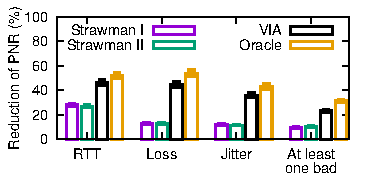
\includegraphics[width=0.5\textwidth]{figures/Via-Eval-Bar-MinChoices-5-Improvement-PNR.pdf}
        \label{subfig:eval-pnr}
}%\hspace{-0.5cm}
\subfloat[\hybrid improvement on percentiles]
{
        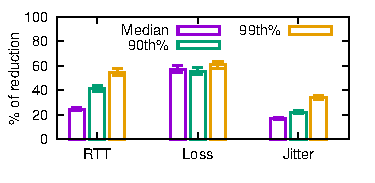
\includegraphics[width=0.5\textwidth]{figures/Via-Eval-Bar-MinChoices-5-Improvement-Percentile.pdf}
        \label{subfig:eval-perc}
}
%\vspace{-0.1cm}
%\hspace{-0.5cm}
\caption{Improvement of \hybrid. PNR on individual metrics improve by $39\%-45\%$ and on the "at least one bad" metric by $23\%$.}
\label{fig:eval-overall}
\end{figure}

\subsection{Improvement of VIA}
\label{subsec:eval-overall}

%\myparatight{Improvement on percentiles}
%Figure~\ref{fig:eval-overall} compares the performance distribution under different relay selection strategies, including ``\direct'' (always using the \direct paths), \hybrid, and the oracle logic (introduced in \Section\ref{sec:potential}). We also compare \hybrid with strawman solutions of predictive and exploratory strategies (discussed in \Section\ref{subsec:hard})\jc{names of strawmen should be changed accordingly when section 4 is done}. 
%From the figures, we can see that across all three performance metrics, \hybrid achieves close-to-oracle performance and significantly outperforms direct paths and strawmen, especially on the high tails. 
%There is \fillme\% to \fillme\% improvement at $90^{\textrm{th}}$\%ile, and \fillme\% to \fillme\% improvement at $99^{\textrm{th}}$\%ile.
%At the same time, we see that the strawman solutions have few improvements, which qualitatively confirms inefficiency of basic predictive strategies or exploratory strategies (\Section\ref{subsec:hard}).


\mypara{PNR reduction}
Figure~\ref{subfig:eval-pnr} shows the PNR reduction of \hybrid over \direct strategy (always using \direct paths), and compares it with the PNR reduction of {pure} prediction-based {selection, based just on history} (Strawman I), {pure} exploration-based selection {without any pruning of the options up front}  (Strawman II), and oracle. 
Across all three performance metrics, we see that \hybrid achieves close-to-oracle performance and significantly outperforms both the default strategy and the two strawman approaches. 
%\sout{At the same time, we see that} 
The strawman approaches yield much less improvement, which confirms the inefficiency of the {pure} predictive and {pure} exploratory strategies (Section~\ref{subsec:strawmen}).

\mypara{Improvement on percentiles} 
Figure~\ref{subfig:eval-perc} shows the improvement over \direct strategy on different percentiles.  
We first calculate the percentiles of performance of each strategy and calculate the improvement between these percentiles (which avoids the bias of calculating improvement on each call).
%The improvement on each percentile is calculated based on the percentile of extrapolated performance of all calls under different strategies (e.g., $90^{\textrm{th}}\%$ of RTT under \hybrid vs. $90^{\textrm{th}}\%$ of RTT under \direct). \vnp{unclear}  
We see that \hybrid has improved performance on both median (by $20\%-58\%$) and {the extreme} tail (by $20\%-57\%$ on $90^\text{th}$ percentile), which shows \hybrid is able to improve the performance of a wide spectrum of calls. % performance.
%\cameraremove{\myparatight{Component-wise contribution:}}

\mypara{Transit vs. bouncing relay} 
%As argued in \Section\ref{??}, an advantage of managed overlays compared to traditional overlays is that a call can avoid WAN routing by going through the backbone of the managed overlay. We define this as ``transport'' relaying, as opposed to ``bouncing'' relaying, where only one relay is used.
Finally, we find that also using transit relaying (i.e., using inter-DC connection between the {ingress and egress relays} as part of the path) usually results in higher improvement on PNR than only using bouncing relays (i.e., using one relay node to bounce off traffic). On AS pairs which have used both bouncing and transit relays, we see $50\%$ {lower} PNR when both transit and bouncing relays are available than when transit relays are excluded.
We also find that \hybrid sends about $54\%$ calls to bouncing relays, $38\%$ to transit relays, $8\%$ to \direct paths, with a marginal difference {in the distribution} across network metrics.

%\begin{figure}[t!]
%\captionsetup[subfigure]{justification=centering,farskip=-1pt,captionskip=-1pt}
%\centering
%%\hspace{-0.5cm}
%\subfloat[Prediction accuracy of tomography.]
%{
%        \includegraphics[width=0.35\textwidth]{new-figs/Tomography-error-CDF.pdf}
%        \label{subfig:eval-component-tomography}
%}\\%\hspace{-0.5cm}
%\subfloat[Various guided-exploration strategies.]
%{
%        \includegraphics[width=0.35\textwidth]{new-figs/Eval-Bar-MinChoices-5-VIA-ComponentWise-PNR.pdf}
%        \label{subfig:eval-component-ucb}
%}\vspace{-0.1cm}
%%\hspace{-0.5cm}
%\tightcaption{Component-wise analysis of \hybrid.}
%\label{fig:}
%\end{figure}

\mypara{International vs. domestic} Figure~\ref{fig:eval-inter-intra} compares PNR of international and domestic calls under strategies of \direct, \hybrid and oracle.%~\footnote{Bars in Figure~\ref{fig:eval-inter-intra} representing the \direct strategy are slightly different from those in Figure~\ref{subfig:opportunity-international}, because Figure~\ref{fig:eval-inter-intra} focuses on only calls between AS pairs where there are enough calls and have used enough relay options (\xref{subsec:eval-method})}.
We see significant improvement of \hybrid on both international and domestic calls, while international calls have a slightly higher magnitude of improvement than domestic calls. 
%We also have similar observation with respect to international calls and domestic ones. 
This can be explained by the fact that relaying has limited benefits when the bottleneck is the last-mile ISP or the last-hop connection.

%\begin{figure}[t!]
%\centering
%\hspace{-0.5cm}
%\subfloat[Inter-domain]
%{
%        \includegraphics[width=0.25\textwidth]{new-figs/Eval-Bar-Interdomain-MinChoices-5.pdf}
%        \label{subfig:}
%}\hspace{-0.5cm}
%\subfloat[Intra-domain]
%{
%        \includegraphics[width=0.25\textwidth]{new-figs/Eval-Bar-Intradomain-MinChoices-5.pdf}
%        \label{subfig:}
%}\hspace{-0.5cm}
%\tightcaption{Inter-domain vs. intra-domain. We see that \hybrid achieves improvements on both inter-domain and intra-domain calls, with a slightly higher magnitude improvement on inter-domain calls. We also have similar observation regarding international and domestic calls. \jc{Figure of international vs. domestic can be added if needed.}}
%\label{fig:eval-inter-intra}
%\end{figure}


\begin{figure}[t!]
\centering
%\hspace{-0.5cm}
\subfloat[International]
{
        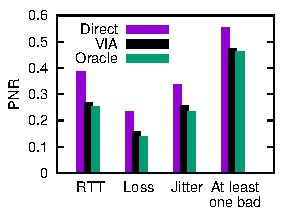
\includegraphics[width=0.45\textwidth]{figures/Via-Eval-Bar-International-MinChoices-5.pdf}
        \label{subfig:eval-international}
}%\hspace{-0.5cm}
\subfloat[Domestic]
{
        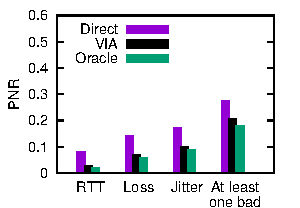
\includegraphics[width=0.45\textwidth]{figures/Via-Eval-Bar-Domestic-MinChoices-5.pdf}
        \label{subfig:eval-domestic}
}%\hspace{-0.5cm}
\caption{\hybrid improvement on international and domestic calls. 
%We see that \hybrid achieves improvements on both international and domestic calls, with a slightly higher magnitude improvement on international calls. 
We also have similar observation regarding inter-domain and intra-domain calls.}
\label{fig:eval-inter-intra}
\end{figure}


\mypara{Benefits by countries} 
Figure~\ref{fig:eval-by-name} further dissects the improvement of \hybrid by countries (with one side of the international call in that country) with worst (direct) PNR. It shows that the worst countries have a much higher (direct) PNR than the global PNR, shown by the horizontal red line, and that the performance of \hybrid is closer to the oracle than to the default for most of these countries. 


%\cameraremove{Figure~\ref{fig:eval-by-name} further dissects the improvement of \hybrid by specific countries and ASes. It shows that many countries and ASes have a much higher PNR than the global PNR (shown by the horizontal red line), and that {the performance of} \hybrid 
%{is closer to the oracle than to the default for} most of these countries and ASes. \camera{Though the figures only show the results for RTT, we also have qualitatively similar observations for the other metrics.}
%
%{That said, }there is also a substantial {disparity in the performance} improvement due to \hybrid for different countries and ASes. 
%Such difference can be explained by how relay nodes are deployed today. For instance, inter-domain calls from AS4766 and AS27947 both suffer from high RTT, but \hybrid is able to improve performance for AS4766 much more {significantly} than for AS27947, because AS4766 has direct peering connection with some relay nodes unlike AS27947.}

\begin{figure}[t!]
\centering
\subfloat[PNR of RTT]
{
        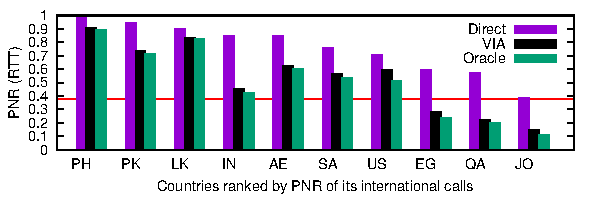
\includegraphics[width=0.75\textwidth]{figures/Via-Eval-Bar-InternationalByCountrySource-MinChoices-5-rRTT.pdf}
        \label{subfig:by-country}
}
%\vspace{-0.4cm}
\\
\subfloat[\small{PNR of loss rate}]
{
        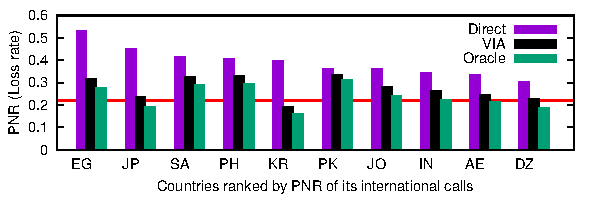
\includegraphics[width=0.75\textwidth]{figures/Via-Eval-Bar-InternationalByCountrySource-MinChoices-5-rLOSS.pdf}
        \label{subfig:by-country}
}
%\vspace{-0.4cm}
\\
\subfloat[PNR of jitter]
{
        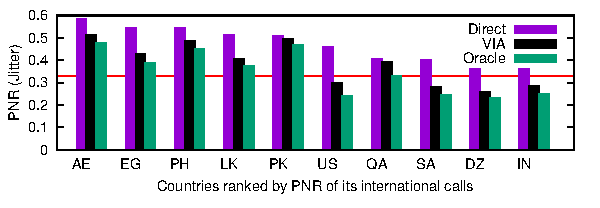
\includegraphics[width=0.75\textwidth]{figures/Via-Eval-Bar-InternationalByCountrySource-MinChoices-5-rJITTER.pdf}
        \label{subfig:by-country}
}
%\vspace{-0.2cm}
%\\
%\subfloat[Inter-domain calls grouped by AS of one side]
%{
%        \includegraphics[width=0.45\textwidth]{new-figs/Eval-Bar-InterdomainByAsnSource-MinChoices-5-rRTT.pdf}
%        \label{subfig:by-asn}
%}
%\tightcaption{Dissecting \hybrid improvement on PNR of RTT by country and AS of one side. There is a substantial diversity on \hybrid improvement across different countries and ASes. }
\caption{Dissecting \hybrid improvement on PNR by country of one side. There is a substantial diversity on \hybrid improvement across different countries. }
\label{fig:eval-by-name}
\end{figure}





%\begin{figure}[t!]
%\centering
%\subfloat[Interdomain calls grouped by source ASes]
%{
%        \includegraphics[width=0.5\textwidth]{new-figs/Eval-Bar-InterdomainByAsnSource-MinChoices-5-rRTT.pdf}
%        \label{subfig:}
%}
%\subfloat[Intradomain calls of different ASes]
%{
%        \includegraphics[width=0.5\textwidth]{new-figs/Eval-Bar-InterdomainByAsnSource-MinChoices-5-rJITTER.pdf}
%        \label{subfig:}
%}
%\tightcaption{Partitioning calls into finer-grained levels. We see a substantial diversity of performance gains between interdomain (or intradomain) calls of different ASes. }
%\label{fig:eval-spatial-partition}
%\end{figure}

\subsection{VIA's Design Choices}
\label{subsec:design}

\mypara{Prediction accuracy of relay-based tomography} 
As a first step, \hybrid uses relay-based tomography (Section~\ref{subsec:practical-prediction}) to predict the performance each \option.
We evaluated the accuracy of tomography-based predictions on the different metrics and found that on $71\%$ of calls, the predicted performance is within $20\%$ from the actual performance. However, for $14\%$ of the calls, the error can be $\geq 50\%$. This non-negligible prediction error explains the poor performance of Strawman I (pure prediction-based) that we have seen in Figure~\ref{subfig:eval-pnr}, and also motivates real-time exploration.





\mypara{Benefits of prediction-guided exploration} 
As discussed in Section~\ref{sec:via:design}, \hybrid is not a simple combination of prediction and exploration approach. 
First, instead of picking a fixed number top candidates, \hybrid pick top candidates by taking variance of prediction into account. 
Second, instead of using the original UCB1 algorithm, which assumes a normal distribution of rewards, we adopt a different way to normalize values to cope with performance outliers.
Figure~\ref{fig:eval-component-ucb} quantifies the incremental contribution of both modifications on PNR of the three metrics.
It shows that each modification makes a significant contribution to \hybrid's improvement. With the ``at least one bad'' metric, picking top $k$ and using the normalized reward reduces PNR by $24\%$ compared to $15\%$ with just the top $2$ (loss rate PNR by $44\%$ compared to $26\%$).
%the improvement of PNR from $26\%$ to $30\%$ ($15\%$ to $17\%$), and using our normalized reward, instead of standard UCB1, further raises the improvement of PNR to $44\%$ (to $23\%$).




%\subsection{Budget constraints}
%\label{subsec:eval-budget}

\subsection{Practical Relaying Factors}
\label{subsec:eval-parameter}



\mypara{Relaying budget} Being able to use relays judiciously within a budget for relayed calls is an inherent requirement in the context of managed overlay networks such as \hybrid. 
Here, we define budget as the maximum fraction of calls being relayed. {We only impose an overall budget, not a per-relay one.}
Figure~\ref{fig:eval-budget} shows the impact of budget on PNR (of at least one bad metric) of three strategies: oracle, budget-unaware \hybrid and budget-aware \hybrid. The budget-unaware \hybrid, which selects relays based on Algorithm~\ref{alg:hybrid}, will relay calls whenever there is potential benefit of doing so, without taking into consideration the overall budget {of relaying}. Therefore, there is a risk of the budget getting used up by calls with only small benefit.
%\vnp{Is there the risk of the budget getting filled up by unimportant calls?} 
In contrast, budget-aware \hybrid (Section~\ref{subsec:practical-budget}) relays a call only when the benefit is larger than a threshold, which depends on the actual budget. That means calls with minimal benefit will not be relayed, saving resources for the calls that would benefit the most by relaying.
From Figure~\ref{fig:eval-budget}, we see that the budget-aware \hybrid (Section~\ref{subsec:practical-budget}) can use budget much more efficiently than the budget-unaware \hybrid. 
Also, budget-aware \hybrid can achieve about half of the maximum benefit (i.e., when budget is $100\%$ of calls) with a budget of $0.3$ (i.e., only relying $30\%$ of calls).%\vnp{why not just stick to percentages, e.g., 30\% instead of 0.3, just to be consistent with an earlier section?}

\begin{figure}[t!]
\centering
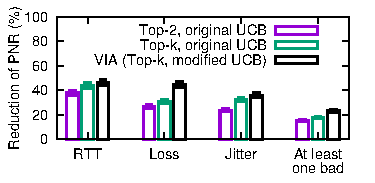
\includegraphics[width=0.5\textwidth]{figures/Via-Eval-Bar-MinChoices-5-VIA-ComponentWise-PNR.pdf}
%\vspace{-0.3cm}
\caption{Comparing guided-exploration strategies.}
\label{fig:eval-component-ucb}
\end{figure}

\begin{figure}[t!]
\centering
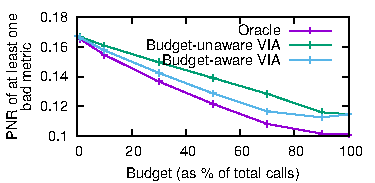
\includegraphics[width=0.5\textwidth]{figures/Via-Eval-Budget-Overall-MinChoices-5-sRTT.pdf}
\caption{Impact of budget constraint on \hybrid.}
\label{fig:eval-budget}
\end{figure}




%So far, we have evaluated \hybrid with a default set up of the managed overlay, where we have no limit on maximum number of relayed calls, and we can leverage all relays.
%Next, we show how the benefit of \hybrid can be affected by various aspect of the managed overlay, including how frequently the relay decisions are made and which relays are used.

\mypara{Relaying decision granularities}
We show performance improvement as a function of the spatial and temporal granularity at which \hybrid operates. 
First, to show the impact of spatial granularity, Figure~\ref{subfig:granularity-spatial} fixes the temporal granularity to running stage ($2$) and ($3$) of \hybrid every $24$ hours, i.e., $T=24$ hours (Figure~\ref{fig:intuition}) 
%\vnp{need to state clearly exactly which part is run every 24 hours}
 and compares the PNR if {different} relay options {could be} selected for calls in different spatial granularities. For fair comparison, the PNR are calculated based on the same set of calls.
%We show {\em PNR inflation} (dividing PNR by the PNR of making decision per AS pair every 24 hours) as a function of spatial granularities of decision making. 

We see two consistent trends. First, making decision at granularities coarser than a per AS pair results in a smaller reduction in PNR. For instance, different ISPs within a country have different peering relationships, and thus may have different optimal relay options, but such opportunities will not be exploited when making decision per country. Second, making decisions on finer granularities does not help much, though for a different reason. At finer granularities, the coverage becomes much smaller, which make \hybrid unable to predict many potential relay options.
In future work we hope to analyze a much larger data set
In Figure~\ref{subfig:granularity-temporal}, we see a similar pattern when comparing PNR of different temporal granularities, i.e., different values of $T$ (Section~\ref{subsec:Via-approach}).  
%\jc{Do we want to claim that AS pair + 24hr is a sweet point?} \ga{Need a better explanation for the second trend.} \vnp{perhaps say that in future work we hope to analyze a much larger data set}

\begin{figure*}[t!]
\centering
\hspace{-0.5cm}
\subfloat[Impact of spatial granularity]
{
        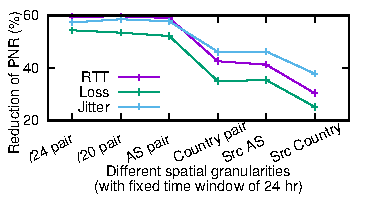
\includegraphics[width=0.5\textwidth]{figures/Via-Eval-Granularity-Spatial.pdf}
        \label{subfig:granularity-spatial}
}
\subfloat[Impact of temporal granularity]
{
        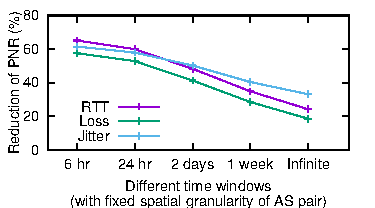
\includegraphics[width=0.5\textwidth]{figures/Via-Eval-Granularity-Temporal.pdf}
        \label{subfig:granularity-temporal}
}\\
\subfloat[Impact of relay deployment]
{
        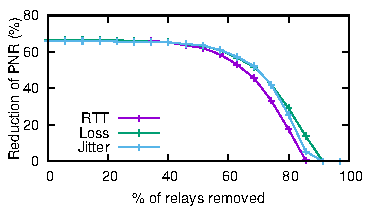
\includegraphics[width=0.5\textwidth]{figures/Via-Eval-Removing-Relays.pdf}
        \label{subfig:eval-deployment}
}
%\hspace{-0.5cm}
\caption{Sensitivity analysis of \hybrid improvement. 
Figure~\ref{subfig:granularity-spatial} and \ref{subfig:granularity-temporal} compares PNR under different control granularities. Figure~\ref{subfig:eval-deployment} shows PNR when some of the (least used) relays are excluded.}
\label{fig:eval-granularity}
\end{figure*}


\mypara{Relay usage} 
Figure~\ref{subfig:eval-deployment} shows reduction of PNR when a subset of (least used) relays is excluded. We see that the contribution of benefits from different relay nodes are highly skewed. Removing $50\%$ of the (least used) relays causes little drop in \hybrid's gains. This suggests that new relays should be deployed carefully in future. 

%\begin{figure}[t!]
%\centering
%\includegraphics[width=0.35\textwidth]{new-figs/Eval-Removing-Relays.pdf}
%\tightcaption{PNR inflation when $n$ least used relays are excluded. We see that the least used 30 relay nodes contributes a tiny fraction of benefit compared with the most used 30 relays nodes.}
%\label{fig:eval-deployment}
%\end{figure}


%Figure~\ref{fig:eval-turnturn} compares the PNR of direct paths, using only bouncing relays (and direct paths), and using all three of bouncing, transport and direct paths. For a fair comparison, we focus on the AS pairs where both bouncing relaying and transport relaying are available. To get the PNR of using only bouncing relays, we run \hybrid algorithm and set the budget of relay options that involve two relays to be zero. 
%We see that though using only bouncing relays can achieve substantial improvement over direct paths, using transport relay can further reduce PNR, especially on loss rate. \jc{We need to say something to justify the marginal additional benefit of transport -- this is really due to the fact that NGC only uses transport relaying in rare cases, which make it hard to even stitch together a transport path in anyway.}

%
%\begin{figure}[t!]
%\centering
%\includegraphics[width=0.35\textwidth]{new-figs/Eval-Bouncing-vs-turnturn.pdf}
%\tightcaption{Comparing PNR of direct paths, using only bouncing relays (and direct paths), and using all three of bouncing, transport and direct paths. We see that though using only bouncing relays can achieve substantual improvement over direct paths, using transport relay can further reduce PNR, especially on loss rate.}
%\label{fig:eval-turnturn}
%\end{figure}

\subsection{Real-World Controlled Deployment}

%The data-driven evaluation (\xref{subsec:eval-method}) we have been using so far is fundamentally limited by two factors -- (1) Since we are not in a position to change the \skype client, it is infeasible to verify how much an {\em individual} caller-callee pair can benefit from using a different relay selected by \hybrid, and (2) Since it is impractical to ask valuable clients to use arbitrary relays, we are not able to quantify the {\em full} potential of \hybrid.
%In this part, we use a controlled experiment platform to address these concerns, though at a very small scale. 
%The platform implements all the key components of \hybrid (\xref{subsec:arch}). We deploy instrumented \skype clients in five countries, and use a centralized controller to instrument the client pairs to make calls using specific \option (\direct paths, bouncing relays or transit relays). 
%After each call, the measured statics of RTT, jitter, and loss are sent back to the controller to inform further decisions.
%Essentially, the controlled experiment platform allows us to measure the performance of the same caller-callee pair on many \options (including those not tried in our dataset) at roughly the same time (e.g., within an hour) and verify the effectiveness of \hybrid (albeit at a very small scale). 

We implemented and deployed a prototype containing the relevant components of \hybrid at a small scale using modified \skype clients and using {\skype}'s production relays. The central controller of our prototype (Figure~\ref{fig:mdn-overview}), deployed on the public Microsoft Azure cloud, aggregated performance measurements from instrumented \skype clients and implemented the relay selection algorithm. The instrumented \skype clients contacted the controller to decide which of the relays of \skype, if any, to use for their calls. We deploy the instrumented client on $14$ machines across Singapore, India, USA, UK and Sri Lanka. Overall, we required minimal modifications to the \skype client.

The controller also orchestrated each client to make calls to the other clients. In total, it created around 1000 calls between $18$ caller-callee pairs. Specifically, it instructed each caller-callee pair to make (short) back-to-back calls using $9-20$ different \options, $4-5$ times each. Since our testbed is at a small scale, such back-to-back calling provides us with high density performance samples between source-destination pairs through many different relays.  We use these samples to perform a controlled experiment on {\hybrid}'s relaying heuristic with accurate ground truth. For simplicity, we omit the direct path as an option.

The results are shown in Figure~\ref{fig:real-world}, where each curve shows the CDF of ``sub-optimality'' of \hybrid's performance on each call, defined by $\frac{\text{Perf}_{\hybrid}-\text{Perf}_{\text{oracle}}}{\text{Perf}_{\text{oracle}}}$.
We found that {\hybrid}'s relaying decision is within $20\%$ of an oracle's performance for $70\%$ of the calls. Note that this is despite picking the {\em best} relay (i.e., sub-optimality of $0$) for no more than $30\%$ of the calls. When there are multiple relaying options with similar performance, temporal fluctuations may lead to not always picking the best option. But \hybrid usually picks the option that is close in performance to the best.
%\cameraremove{We find that {\hybrid}'s relaying decision is within $5\%$ of an oracle's performance for more than $95\%$ of the calls.}


\begin{figure}[t!]
\centering
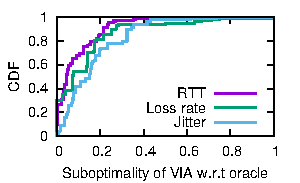
\includegraphics[width=0.45\textwidth]{figures/Via-Rajdeep-active-exp-CDF.pdf}
\caption{Deployment results. CDF, over calls, of sub-optimality (lower is better) of \hybrid's performance.}
\label{fig:real-world}
\end{figure}


%\commentout{
%\camera{
%\begin{table}[t!]
%\centering
%\begin{footnotesize}
%\begin{tabular}{ccccc}
%   Pairs    & Location & Oracle & \hybrid & Default \\ \hline\hline
%Pair A & N. America - S. Asia & 235    & 248 & 282     \\ \hline
%Pair B & N. America - S.E. Asia & 252      & 254  & 269      \\ \hline
%Pair C & S. Asia - S.E. Asia & 45   &  46 &     45
%\end{tabular}
%\end{footnotesize}
%\tightcaption{Example of real-world validation results. Each cell represents the average RTT (ms) of each strategy.}
%\label{tab:real-world}
%\end{table}
%
%\camera{To provide more detail results of the controlled experiments, Table~\ref{tab:real-world} compares the average RTT of \hybrid strategy, \direct path and oracle strategy on three specific client pairs. We pick these client pairs as they represent distinct geographical characteristics -- Pair A is between two long distance wireless clients, Pair B is between two long distance Ethernet clients, and Pair C is between (relatively) short distance clients. 
%While \hybrid achieves close-to-optimal performance, we also make two interesting observations pertaining to the nature of these client pairs.
%First, one would expect it is more likely for \hybrid to find the best \option for Pair A than for Pair B, because the performance gap between the best relay (i.e., Oracle) and \direct path of Pair A (235ms vs. 282ms) is much larger than Pair B (252ms vs. 269ms). Yet, \hybrid's performance is closer to optimal on Pair B than on Pair A, because Pair A is between two wireless clients, whose noisy performance makes it more difficult for \hybrid to identify the best decisions for Pair A than for Pair B (which is between ethernet clients).
%Second, the fact that the \direct path is the best choice for Pair C while using certain relay is the best for Pair A and B echoes one of the observations in \S\ref{sec:motivation} that long-distance calls benefit more from relaying. 
%}
%}
%
%
%%The data-driven evaluation (\xref{subsec:eval-method}) we have been using so far is unable to estimate how much an {\em individual} caller-callee pair can benefit if it were to use the relay selected by \hybrid that was not used by it in the dataset. 
%%Since for now, we are not in a position to change the \skype client, this is a fundamental limitation of using passively collected measurements.
%%In this part, we use a controlled experiment platform to address this concern, though at a very small scale. 
%%The platform implements all the key components of \hybrid (\xref{subsec:arch}). We deploy instrumented \skype clients in five countries, and use a centralized controller to instrument the client pairs to make calls using specific \option (\direct paths, bouncing relays or transit relays). 
%%After each call, the measured statics of RTT, jitter, and loss are sent back to the controller to inform further decisions.
%%
%%Essentially, the controlled experiment platform allows us to measure the performance of the same caller-callee pair on many \options at roughly the same time and verify the effectiveness of \hybrid (albeit at a very small scale).
%%Specifically, we let each pair of caller and callee to make back-to-back calls (each of 2 minutes) using 10 different \options. This provides the performance measurements of 10 \options for the same caller-callee pair at roughly the same time (i.e., within 20-minute window).
%%Then, we repeat this process for multiple rounds, to get this complete set of measurements over a period of time. Based on this dataset, we can evaluate the behavior of \hybrid more accurately.
%%
%%Table~\ref{tab:real-world} compares the average RTT of the \options selected by \hybrid with that of \direct and oracle strategies. 
%%%The relays are chosen based on geographical proximity (i.e., none of the relays is clearly worse than others in a geographical sense).
%%We choose three client pairs as each of them represents a unique scenario.
%%Pair A and Pair B are long-distance calls, while Pair C has relatively shorter distance calls. Furthermore, Pair A is between two wirelessly connected home machines, and Pair B is between two wiredly connected campus machines. Note that such case study with machine-specific information is rarely feasible in the passively measured dataset.
%%Overall, we see that \hybrid is able achieve close-to-optimal performance.
%%In addition, there are two observations pertaining to the nature of each pair. 
%%(1) The fact that the direct path is the best choice for Pair C while using certain relay is the best for Pair A and B reinforces the observation that relay has a larger benefit on long-distance calls. 
%%(2) Pair A has a larger performance gap between its best relay path and the \direct path than Pair B does, which seems to suggest \hybrid should identify the best relay of Pair A more easily. Interestingly, we see that \hybrid has more close-to-optimal performance on Pair B than on Pair A. This is because Pair A (whose end points are wireless connection) has larger performance variation than Pair B (whose end points are wiredly connected), which makes it relatively more difficult for \hybrid to identify the better decision.
%}
%We also see that despite the geographical proximity, some relay options have even worse performance than others and the \direct path, suggesting that data-driven relay selection is necessary.
%In addition, we find a substantial variation of performance even on the same caller-callee pair using the same \option within an hour (figure omitted), which reinforces that the challenge of performance variability (\xref{subsec:strawmen}) is inherent.

%\jc{Venkat, do you think the second part is necessary?}
%Second, several relay options our experiments have not been used in our dataset (either because it was not deployed or due to incrementality in the deployment). We see that these relay options in general have similarly good performance to others, and sometimes, even better. 
%This makes a case for \skype production system to deploy \hybrid to select relays over a large pool of relay choices, which would both benefit the performance and increase the budget for relayed calls (which as \xref{subsec:eval-budget} shows, has significant benefit on performance).


%\subsection{Real-world validation}
%\jc{Two messages:
%\begin{packeditemize}
%\item Validate the best relays chosen by the offline decision-making algorithm. Basically, I can provide Rajdeep with a list of best relay options from the set of relays visible to me, and we can check how close is the real performance of the relay recommended by me and that of the best relay found in Rajdeep's dataset. If the gap is too large, we can compare it with the best relay among the same set of relays (I.e., both Rajdeep and I choose relay from the set of relays visible to me).
%\item Evaluate performance of other relay options that haven't been tried (this may bring a little contradiction to section 3), and say we are deploying this system in an incremental manner, and there would larger improvement with more complete deployment.
%\end{packeditemize}}






\section{Discussion}
\label{sec:via:discussion}

\mypara{Cost of centralized control in \hybrid} Our pilot deployment and client modifications suggest a feasible path to a large-scale deployment from a software update and engineering perspective. One potential concern, however, is the scalability and responsiveness of the control platform. On the one hand, {\hybrid} introduces minimal per call overhead, since the client-controller communication need only consist of one measurement update and one control message exchange per call and can be further reduced if the clients cache the best relaying options. % On the one hand, it leads to additional measurement updates and control messages sent between clients and controller, but the overhead might be acceptable given that the update/control messages would only be one per call, and that can be further reduced if the clients can cache the best relaying options. 
On the other hand, handling a large number of call connections at one logical controller presents a scalability challenge, though partitioning techniques provide a good starting point. Also, we conjecture that approaches similar to the split-control architecture employed in C3~\cite{c3} might offer a scalable realization, since the measurement and control exchange of the C3 controller (which directs clients to video CDNs) is similar to the measurement and control needed for a large-scale VOIP relay server. 


\mypara{Hybrid reactive decentralized approaches} A natural alternative to relay selection is to simply have clients try a list of relay options sequentially or in parallel, and pick the best option. Such an approach may be good enough for long-lived calls. This would avoid the overhead of data collection and generating the network map. However, as we discussed earlier, this may not be feasible given the large search space of relaying options. An interesting hybrid approach is using the prediction-guided exploration observations as a means to {\em prioritize or prune} this approach. We intend to explore this approach going forward.

\mypara{Active Measurements} While our current solution relied entirely on passive measurements from client calls, there is an opportunity to augment it with {\em active} measurements (by making mock calls between users or from users to relays), especially since the client software can be readily controlled to make them. Active measurements can be intelligently orchestrated to fill ``holes'' in the passively obtained measurements, thereby making our prediction-guided exploration (both its aspects---tomography as well as bandit solution) more effective. Doing so will require considering the additional load imposed on the clients due to the collection. 









\section{Related Work}
\label{sec:via:related}


\mypara{Overlay routing}
Overlay networking has been explored in a variety of contexts, such as virtual private networks (VPNs) and multicast~\cite{mbone,ALMI-USITS01,Multicast-Sigcomm02}. Of interest to us here is work focused on overlay routing with a view to improving performance~\cite{Detour-Sigcomm99,RON-SOSP01}. This work showed that performance in terms of network metrics such as delay and packet loss, and also reliability, could be improved by using an overlay path that traverses well-chosen waypoints. 

Despite this promise,  overlay routing for performance gains has not seen much adoption in practice, for several reasons including the last-mile performance bottlenecks encountered in using client nodes as peers and the policy issues involved in turning stub networks (e.g., university campus networks) into de facto transit networks. Perhaps most importantly, these efforts involved building up overlay networks from scratch, both in terms of physical infrastructure and network probing, which limited their scale.

Our work revisits the idea of overlay routing in the context of (a) global-scale managed networks, so the global infrastructure already exists and need not be built up from scratch, and (b) a large-scale interactive real-time service, \skype, which provides both a compelling need for improving performance and (passive) measurements to obviate the need for active network probing.


\mypara{Evolution of AV conferencing services} The architecture of audio-video conferencing services has been evolving, with a trend towards leveraging cloud resources. A case in point is Skype, which started off with a peer-to-peer approach to NAT and firewall traversal, with some well-connected clients with public IP addresses serving as super-nodes~\cite{Skype-GI08}. However, in the recent years, Skype has moved to a hybrid model~\cite{VideoTelephony-IMC12}, with some super-nodes hosted in the cloud~\cite{Skype-Zdnet13}. 
It has been reported that Google Hangouts uses relays in the cloud for all calls, and moreover also has streams traverse the cloud backbone from one relay to another~\cite{VideoTelephony-IMC12}. 

Our work is in line with these trends, but focused on performance rather than NAT/firewall traversal. Also, since we focus on managed networks, being selective in which streams are routed via the cloud is crucial in our context.

\mypara{CDN server selection} Optimal server selection is a much-studied problem, especially in the context of content distribution networks \cite{DONAR-Sigcomm10,youtubecdn}. The main considerations in the selection process are typically proximity of the client to replicas and the load on the replicas. The main distinction of our work is our focus on client-to-client communication, which means that relay selection needs to focus on end-to-end performance rather than just between the cloud edges and the client.

\mypara{Internet performance prediction} There is a large body of work on Internet performance prediction~\cite{IDMaps-ToN01,GNP-Infocom02,iplaneosdi}, with a focus on metrics such as bandwidth, delay, and packet loss rate. The general approach is to probe the network selectively, at chosen times and along chosen paths, and then to use the measurements to either embed the network nodes in a coordinate space~\cite{dabek2004vivaldi} or estimate the performance of network segments using network tomography techniques~\cite{Tomography-StatSci04}.
 Since we have access to network metrics for a large volume of calls, our work focuses on leveraging this data rather than performing active measurements.


\mypara{Measurement studies} Over the years, there have been a number of measurement studies of large Internet services, including web sites~\cite{Padmanabhan-Sigcomm00},  CDNs~\cite{CDN-OSDI02}, and video-on-demand streaming~\cite{Streaming-Usits01,sigcomm11}. There have also been studies of audio-video conferencing by working outside the system, say by running active measurements to Skype super-nodes~\cite{SkypeMeasurement-IPTPS07} or sniffing traffic in modest-size deployments~\cite{VideoTelephony-IMC12}. 
To our knowledge, this work is the first study of a commercial VoIP service at scale by directly working with end-to-end performance metrics recorded by the communicating peers themselves.

\mypara{Estimating VoIP Quality} Several models have been proposed and studied for estimating VoIP quality, typically the Mean Opinion Score (MOS), based on network performance metrics~\cite{cole,SkypeUserSatisfaction-Sigcomm06,SkypeMeasurement-IPTPS07,SkypeQuality-WMUST12,SkypeQoE-Multimedia12}. These models vary in the particular network metrics and codecs they consider. In Section~\ref{sec:via:potential}, we used the model proposed in ~\cite{cole}, which is based on the E-Model defined by the ITU~\cite{itu-e-model15}. 


\section{Summary}
\label{sec:via:summary}

By some estimates, the call volume of Internet telephony surpasses that 
of traditional telephony. Given its importance, in this chapter, we 
have applied \ddn paradigm to improve VoIP QoE.
To mitigate calls with poor quality, we revisit the classical overlay network 
techniques with the emerging managed networks of large cloud providers. 
Calls between users with poor network conditions can be {\em selectively relayed}
via the managed network.

To leverage such a managed overlay infrastructure, we have presented the 
design of  \hybrid, a system that dynamically select a close-to-optimal relay
path in the managed overlay for each call.
\hybrid addresses a key limitation faced by previous \ddn-based solutions 
(e.g., CFA or Pytheas) in Internet telephony--data sparsity caused by a large
decision space.
The key insight of \hybrid to address this challenge is that, for each pair of caller 
ISP and callee ISP, there is a {\em small and stable subset} of relays that 
almost always contains the best relay.
Inspired by the insight, \hybrid uses a guided 
 exploration procedure using predicted performance 
 derived from end-to-end measurements collected by 
 the clients, while dealing with variances in real-world estimates and keeping 
 the volume of relayed calls within a budget. 
 Data-driven evaluation shows that \hybrid improves call quality by 
 $45\%$ which closely matches the potential benefits indicated by an oracle. 

%By some estimates, the call volume of Internet telephony surpasses that of traditional telephony. 
%Given its importance, we take the first step towards quantifying the impact of network performance on call quality using traces from \skype, one of the largest VoIP services. Our sampled dataset consists of $430$ million calls over seven months. To mitigate calls with poor quality, we revisit the classical overlay network techniques but using the {\em managed} networks of large cloud providers. Calls between users with poor network conditions can be {\em selectively relayed} via the managed network. Such managed overlays do not suffer from the drawbacks of traditional overlays. 
%
%To leverage such a managed overlay infrastructure, we present the 
% design of  \hybrid, a system that carefully selects a subset
% of  calls to be relayed using the managed overlay. \hybrid uses a guided 
% exploration procedure using predicted performance derived from end-to-end measurements collected by the clients, while dealing with variances in real-world estimates and keeping the volume of relayed calls within a budget. Data-driven evaluation shows that \hybrid improves call quality by $45\%$ which closely matches the potential benefits indicated by an oracle. 





